%Figuras
%%%%%%%%%%%%%%%%%%%%%%%%%%%%%%%%%%%%%%%%%trayectoria hamiltoniana%%%%%%%%%%%%%%%
\begin{frame}
\frametitle{Estrategia usual. \hspace{2cm} A}
%\begin{itemize}
%\centering \item \textcolor{blue}{$A$}
%\end{itemize}

\begin{figure}[!ht]
\begin{center}
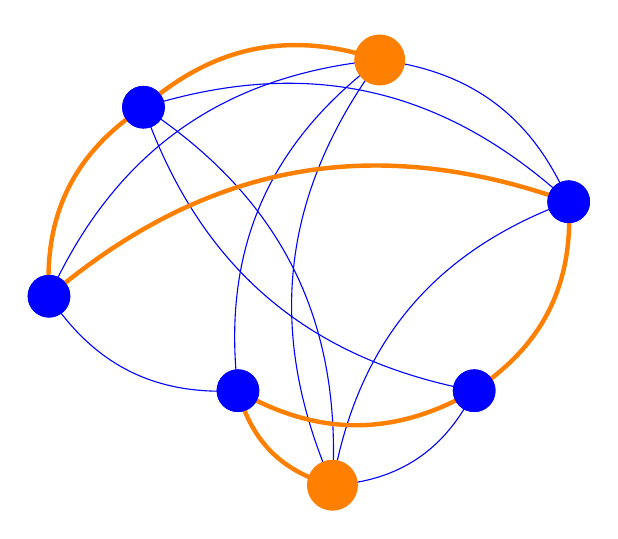
\begin{tikzpicture}[scale=0.3]

\draw[-,color=blue] (14,2) to [bend left] (10,6);
\draw[-,color=blue] (14,2) to [bend right] (20,6);
\draw[-,color=blue] (10,6) to [bend left] (2,10);%
\draw[-, color=blue] (2,10) to [bend left] (6,18);
\draw[-, color=blue] (20,6) to [bend right] (24,14);%
\draw[-, color=blue] (6,18) to [bend left] (16,20);
\draw[-,color=blue] (16,20) to [bend left] (24,14); %

\draw[-,color=blue] (16,20) to [bend right] (2,10);
\draw[-,color=blue] (16,20) to [bend right] (10,6);
\draw[-,color=blue] (6,18) to [bend left] (14,2);
\draw[-, color=blue] (2,10) to [bend left] (24,14);%%
\draw[-, color=blue] (10,6) to [bend right] (20,6);
\draw[-,color=blue] (24,14) to [bend right] (14,2);
\draw[-,color=blue] (16,20) to [bend right] (14,2);
\draw[-,color=blue] (6,18) to [bend right] (20,6);
\draw[-,color=blue] (6,18) to [bend left] (24,14);%
\draw[-, color=blue] (10,6) to [bend right] (14,2);

\filldraw[color=orange] (14,2) circle (30pt);
\filldraw[color=blue] (10,6) circle (25pt);
 \filldraw[color=blue] (20,6) circle (25pt);
 \filldraw[color=blue] (2,10) circle (25pt); 
 \filldraw[color=blue] (6,18) circle (25pt);
 \filldraw[color=blue] (24,14) circle (25pt);
\filldraw[color=orange] (16,20) circle (30pt);

\draw[-, >=latex,ultra thick,color=orange] (6,18) to [bend left] (16,20);

\draw[-, >=latex,ultra thick,color=orange] (2,10) to [bend left] (6,18);

\draw[-, >=latex,ultra thick,color=orange] (2,10) to [bend left] (24,14);

\draw[-, >=latex,ultra thick,color=orange] (20,6) to [bend right] (24,14);%


\draw[-, >=latex,ultra thick,color=orange] (10,6) to [bend right] (20,6);

\draw[-, >=latex,ultra thick,color=orange] (10,6) to [bend right] (14,2);


\filldraw[color=blue] (10,6) circle (25pt);
\filldraw[color=blue] (20,6) circle (25pt);
\filldraw[color=blue] (2,10) circle (25pt); 
\filldraw[color=blue] (6,18) circle (25pt);
\filldraw[color=blue] (24,14) circle (25pt);


\end{tikzpicture}
\end{center}
\end{figure}
\centering 
\end{frame}





%%%%%%%%%%%%%%%%%%%%%%%%%%%%%%%%%%%%%%%%%%%%%%%%%%%%%%%%%%%%%%%%G_n  (verde etiquetado con numeros)$$$$$$$$$$$$$$$$$$$$$$$$$$$$$$$4
\begin{frame}
\frametitle{Transformaci�n $f:G_m \rightarrow G_n$}

\begin{figure}[!ht]
\begin{center}
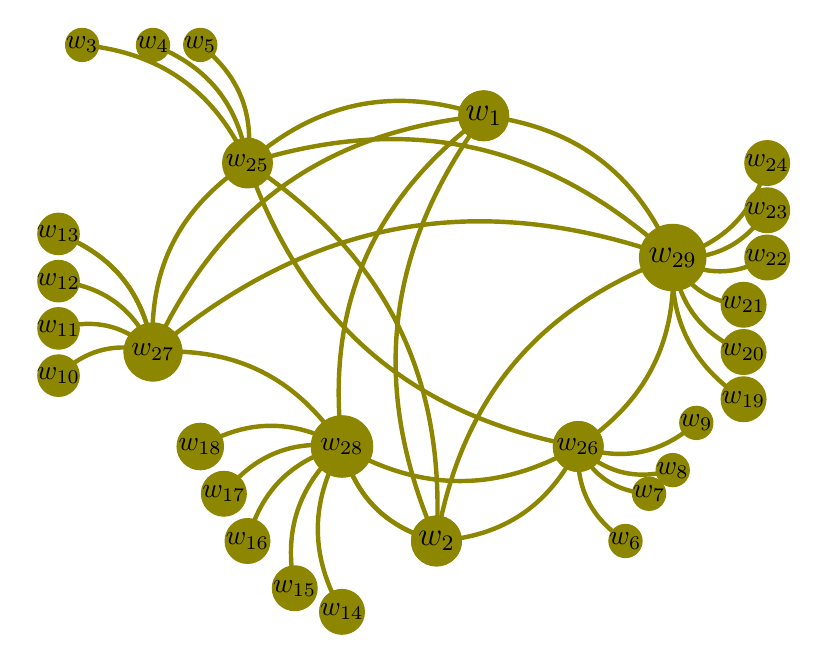
\begin{tikzpicture}[scale=0.3]

\draw[-,>=latex,ultra thick,color=olive] (14,2) to [bend left] (10,6);
\draw[-,>=latex,ultra thick,color=olive] (14,2) to [bend right] (20,6);
\draw[-,>=latex,ultra thick, color=olive] (10,6) to [bend right] (2,10);%
\draw[-,>=latex,ultra thick, color=olive] (2,10) to [bend left] (6,18);
\draw[-, >=latex,ultra thick, color=olive] (20,6) to [bend right] (24,14);%
\draw[-, >=latex,ultra thick, color=olive] (6,18) to [bend left] (16,20);
\draw[-, >=latex,ultra thick, color=olive] (16,20) to [bend left] (24,14); %

\draw[-, >=latex,ultra thick, color=olive] (16,20) to [bend right] (2,10);
\draw[-, >=latex,ultra thick, color=olive] (16,20) to [bend right] (10,6);
\draw[-, >=latex,ultra thick,color=olive] (6,18) to [bend left] (14,2);
\draw[-, >=latex,ultra thick, color=olive] (2,10) to [bend left] (24,14);%%
\draw[-,>=latex,ultra thick, color=olive] (10,6) to [bend right] (20,6);
\draw[-, >=latex,ultra thick,color=olive] (24,14) to [bend right] (14,2);
\draw[-,>=latex,ultra thick, color=olive] (16,20) to [bend right] (14,2);
\draw[-, >=latex,ultra thick,color=olive] (6,18) to [bend right] (20,6);
\draw[-, >=latex,ultra thick, color=olive] (6,18) to [bend left] (24,14);%
\draw[-, >=latex,ultra thick, color=olive] (10,6) to [bend right] (14,2);




\filldraw[color=olive] (14,2) circle (30pt) node[] {\large \textcolor{black}{$v_2$}};
\filldraw[color=olive] (10,6) circle (30pt)node[] {\large \textcolor{black}{\normalsize{$v_{6}$}}};;
 \filldraw[color=olive] (20,6) circle (30pt)node[] {\large \textcolor{black}{$v_4$}};;
 \filldraw[color=olive] (2,10) circle (25pt)node[] {\large \textcolor{black}{$v_5$}}; 
 \filldraw[color=olive] (6,18) circle (25pt)node[] {\large \textcolor{black}{$v_3$}};;
 \filldraw[color=olive] (24,14) circle (25pt)node[] {\large \textcolor{black}{$v_7$}};;
\filldraw[color=olive] (16,20) circle (30pt) node[] {\large \textcolor{black}{$v_1$}};


%%%%%%%%%%%%%%%%%%%%%%%%%%%%%%%%
\filldraw[color=olive] (16,20) circle (30pt) node[] {\large \textcolor{black}{$w_1$}};
%%%%%%%%%%%%%%%%%%%%%%%%%%%%%%%%%%%%%%%%%%%%%
\filldraw[color=olive] (14,2) circle (30pt) node[] {\large \textcolor{black}{$w_2$}};

%%%%%%%%%%%%%%%%%%%%%%%%%%%%%%%%%


\draw[-,>=latex,ultra thick,color=olive] (6,18) to [bend right](-1,23);
\draw[-,>=latex,ultra thick, color=olive] (6,18) to [bend right] (2,23);
\draw[-,>=latex,ultra thick, color=olive] (6,18) to [bend right] (4,23);

\filldraw[color=olive] (-1,23) circle (20pt) node[] {\textcolor{black}{$w_3$}};
\filldraw[color=olive] (2,23) circle (20pt) node[] { \textcolor{black}{$w_4$}};
\filldraw[color=olive] (4,23) circle (20pt) node[] {\textcolor{black}{$w_5$}};

\filldraw[color=olive] (6,18) circle (30pt) node[] { \textcolor{black}{$w_{25} $}};

%%%%%%%%%%%%%%%%%%%%%%%%%%%%%%%%%%%%%%

\draw[-,>=latex,ultra thick, color=olive] (20,6) to [bend right](22,2);
\draw[-, >=latex,ultra thick,color=olive] (20,6) to [bend right] (23,4);
\draw[-,>=latex,ultra thick, color=olive] (20,6) to [bend right] (24,5);
\draw[-,>=latex,ultra thick,color=olive] (20,6) to [bend right] (25,7);

\filldraw[color=olive] (22,2) circle (20pt) node[] {\textcolor{black}{$w_6$}};
\filldraw[color=olive] (23,4) circle (20pt) node[] { \textcolor{black}{$w_7$}};
\filldraw[color=olive] (24,5) circle (20pt) node[] {\textcolor{black}{$w_8$}};
\filldraw[color=olive] (25,7) circle (20pt) node[] { \textcolor{black}{$w_9$}};
%\filldraw[color=olive] (6,18) circle (20pt) node[] {\tiny \textcolor{black}{$w_{k+1}$}};
\filldraw[color=olive] (20,6) circle (30pt) node[] {\textcolor{black}{$w_{26}$}};


%%%%%%%%%%%%%%%%%%%%%%%%%%%%%%%%%%%%%%55
\draw[-,>=latex,ultra thick,color=olive] (2,10) to [bend right](-2,9);
\draw[-,>=latex,ultra thick,color=olive] (2,10) to [bend right] (-2,11);
\draw[-,>=latex,ultra thick,color=olive] (2,10) to [bend right] (-2,13);
\draw[-,>=latex,ultra thick,color=olive] (2,10) to [bend right] (-2,15);
\draw[-,>=latex,ultra thick,color=olive] (2,10) to [bend right] (-2,15);

\filldraw[color=olive] (-2,9) circle (25pt) node[] { \textcolor{black}{$w_{10}$}};
\filldraw[color=olive] (-2,11) circle (25pt) node[] { \textcolor{black}{$w_{11}$}};
\filldraw[color=olive] (-2,13) circle (25pt) node[] {\textcolor{black}{$w_{12}$}};
\filldraw[color=olive] (-2,15) circle (25pt) node[] {\textcolor{black}{$w_{13}$}};


\filldraw[color=olive] (2,10) circle (35pt) node[] {\textcolor{black}{$w_{27}$}};


%%%%%%%%%%%%%%%%%%%%%%%%%%%%%%%55

\draw[-,>=latex,ultra thick,color=olive] (10,6) to [bend right](10,-1);
\draw[-,>=latex,ultra thick,color=olive] (10,6) to [bend right] (8,0);
\draw[-,>=latex,ultra thick,color=olive] (10,6) to [bend right] (6,2);
\draw[-,>=latex,ultra thick,color=olive] (10,6) to [bend right] (5,4);
\draw[-,>=latex,ultra thick,color=olive] (10,6) to [bend right] (4,6);
\filldraw[color=olive] (10,-1) circle (27pt) node[] { \textcolor{black}{$w_{14}$}};
\filldraw[color=olive] (8,0) circle (27pt) node[] { \textcolor{black}{$w_{15}$}};
\filldraw[color=olive] (6,2) circle (27pt) node[] { \textcolor{black}{$w_{16}$}};
\filldraw[color=olive] (5,4) circle (27pt) node[]{ \textcolor{black}{$w_{17}$}};
\filldraw[color=olive] (4,6) circle (28pt) node[] {\textcolor{black}{$w_{18}$}};





\filldraw[color=olive] (10,6) circle (37pt) node[] { \textcolor{black}{$w_{28}$}};

%%%%%%%%%%%%%%%%%%%%%%%%%%%%%%%%%%%%%%%%%%%%%%%%%%
\draw[-,>=latex,ultra thick, color=olive] (24,14) to [bend right](27,8);
\draw[-,>=latex,ultra thick,color=olive] (24,14) to [bend right] (27,10);
\draw[-,>=latex,ultra thick,color=olive] (24,14) to [bend right] (27,12);
\draw[-,>=latex,ultra thick,color=olive] (24,14) to [bend right] (28,14);
\draw[-,>=latex,ultra thick,color=olive] (24,14) to [bend right] (28,16);
\draw[-,>=latex,ultra thick,color=olive] (24,14) to [bend right] (28,18);

\filldraw[color=olive] (27,8) circle (27pt) node[] { \textcolor{black}{$w_{19}$}};
\filldraw[color=olive] (27,10) circle (27pt) node[] { \textcolor{black}{$w_{20}$}};
\filldraw[color=olive] (27,12) circle (27pt) node[] { \textcolor{black}{$w_{21}$}};
\filldraw[color=olive] (28,14) circle (27pt) node[] { \textcolor{black}{$w_{22}$}};
\filldraw[color=olive] (28,16) circle (27pt) node[] { \textcolor{black}{$w_{23}$}};
\filldraw[color=olive] (28,18) circle (27pt) node[] {\textcolor{black}{$w_{24}$}};


%\filldraw[color=olive] (6,18) circle (30pt) node[] {\tiny \textcolor{black}{$w_{k+1}$}};
%\filldraw[color=olive] (20,6) circle (30pt) node[] {\tiny \textcolor{black}{$w_{k+2}$}};
%\filldraw[color=olive] (2,10) circle (35pt) node[] {\tiny \textcolor{black}{$w_{k+i-2}$}};
%\filldraw[color=olive] (10,6) circle (37pt) node[] {\tiny \textcolor{black}{$w_{k+m-3}$}};
%\filldraw[color=olive] (24,14) circle (40pt) node[] {\tiny \textcolor{black}{$w_{k+m-2}$}};

\filldraw[color=olive] (24,14) circle (40pt) node[] {\large \textcolor{black}{$w_{29}$}};

\end{tikzpicture}
\end{center}
\end{figure}
\end{frame}

%%%%%%%%%%%%%%%%%%%%%%%%%%%%%%%%%%%%%%%%%%%%%%%%%%%%%%%%%%%%%%%%%%%%%%%%%%%%%%%%%%%%%%%%%%%%%%%%%%%%%%%%%%%%
%%%%%%%%%%%%%%%%%%%%%%%%%%%%%%%%%%%%%%%%%%%%%%% �rbol de G_n (orange)%%%%%%%%%%%%%%%%%%%%%%%%%%%%%%%%%%%%%%%%%

\begin{frame}
\begin{figure}[!ht]
\begin{center}
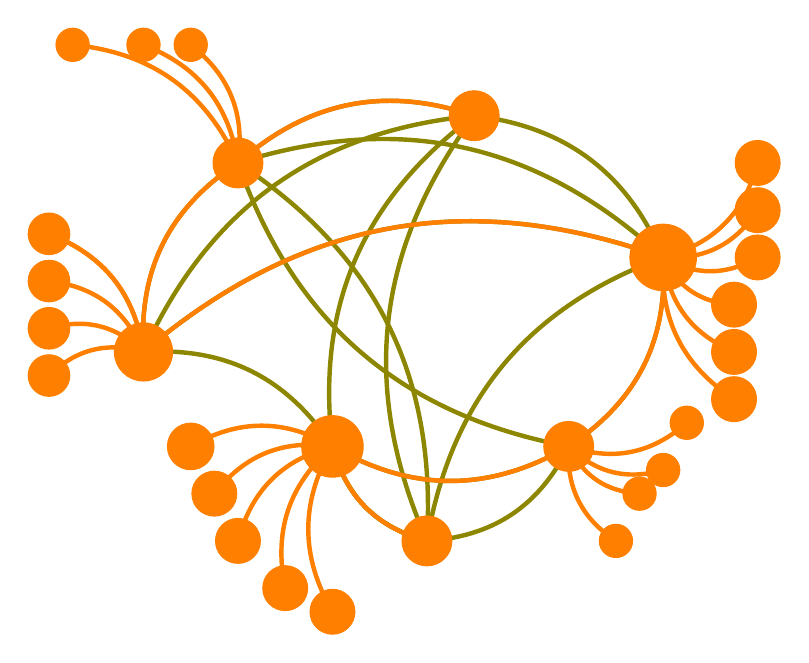
\begin{tikzpicture}[scale=0.3]

\draw[-,>=latex,ultra thick,color=olive] (14,2) to [bend left] (10,6);
\draw[-,>=latex,ultra thick,color=olive] (14,2) to [bend right] (20,6);
\draw[-,>=latex,ultra thick, color=olive] (10,6) to [bend right] (2,10);%
\draw[-,>=latex,ultra thick, color=olive] (2,10) to [bend left] (6,18);
\draw[-, >=latex,ultra thick, color=olive] (20,6) to [bend right] (24,14);%
\draw[-, >=latex,ultra thick, color=olive] (6,18) to [bend left] (16,20);
\draw[-, >=latex,ultra thick, color=olive] (16,20) to [bend left] (24,14); %

\draw[-, >=latex,ultra thick, color=olive] (16,20) to [bend right] (2,10);
\draw[-, >=latex,ultra thick, color=olive] (16,20) to [bend right] (10,6);
\draw[-, >=latex,ultra thick,color=olive] (6,18) to [bend left] (14,2);
\draw[-, >=latex,ultra thick, color=olive] (2,10) to [bend left] (24,14);%%
\draw[-,>=latex,ultra thick, color=olive] (10,6) to [bend right] (20,6);
\draw[-, >=latex,ultra thick,color=olive] (24,14) to [bend right] (14,2);
\draw[-,>=latex,ultra thick, color=olive] (16,20) to [bend right] (14,2);
\draw[-, >=latex,ultra thick,color=olive] (6,18) to [bend right] (20,6);
\draw[-, >=latex,ultra thick, color=olive] (6,18) to [bend left] (24,14);%
\draw[-, >=latex,ultra thick, color=olive] (10,6) to [bend right] (14,2);




%\filldraw[color=olive] (14,2) circle (30pt) node[] {\large \textcolor{black}{$v_2$}};
%\filldraw[color=olive] (10,6) circle (30pt)node[] {\large \textcolor{black}{\normalsize{$v_{6}$}}};;
% \filldraw[color=olive] (20,6) circle (30pt)node[] {\large \textcolor{black}{$v_4$}};;
% \filldraw[color=olive] (2,10) circle (25pt)node[] {\large \textcolor{black}{$v_5$}}; 
% \filldraw[color=olive] (6,18) circle (25pt)node[] {\large \textcolor{black}{$v_3$}};;
% \filldraw[color=olive] (24,14) circle (25pt)node[] {\large \textcolor{black}{$v_7$}};;
%\filldraw[color=olive] (16,20) circle (30pt) node[] {\large \textcolor{black}{$v_1$}};


%%%%%%%%%%%%%%%%%%%%%%%%%%%%%%%%
\filldraw[color=orange] (16,20) circle (30pt);% node[] {\large \textcolor{black}{$w_1$}};
%%%%%%%%%%%%%%%%%%%%%%%%%%%%%%%%%%%%%%%%%%%%%
\filldraw[color=orange] (14,2) circle (30pt);% node[] {\large \textcolor{black}{$w_2$}};

%%%%%%%%%%%%%%%%%%%%%%%%%%%%%%%%%


\draw[-,>=latex,ultra thick,color=orange] (6,18) to [bend right](-1,23);
\draw[-,>=latex,ultra thick, color=orange] (6,18) to [bend right] (2,23);
\draw[-,>=latex,ultra thick, color=orange] (6,18) to [bend right] (4,23);

\filldraw[color=orange] (-1,23) circle (20pt);% node[] {\textcolor{black}{$w_3$}};
\filldraw[color=orange] (2,23) circle (20pt);% node[] { \textcolor{black}{$w_4$}};
\filldraw[color=orange] (4,23) circle (20pt);% node[] {\textcolor{black}{$w_5$}};

\filldraw[color=orange] (6,18) circle (30pt);% node[] { \textcolor{black}{$w_{25} $}};

%%%%%%%%%%%%%%%%%%%%%%%%%%%%%%%%%%%%%%

\draw[-,>=latex,ultra thick, color=orange] (20,6) to [bend right](22,2);
\draw[-, >=latex,ultra thick,color=orange] (20,6) to [bend right] (23,4);
\draw[-,>=latex,ultra thick, color=orange] (20,6) to [bend right] (24,5);
\draw[-,>=latex,ultra thick,color=orange] (20,6) to [bend right] (25,7);

\filldraw[color=orange] (22,2) circle (20pt); %node[] {\textcolor{black}{$w_6$}};
\filldraw[color=orange] (23,4) circle (20pt); %node[] { \textcolor{black}{$w_7$}};
\filldraw[color=orange] (24,5) circle (20pt); %node[] {\textcolor{black}{$w_8$}};
\filldraw[color=orange] (25,7) circle (20pt); %node[] { \textcolor{black}{$w_9$}};
%\filldraw[color=olive] (6,18) circle (20pt) node[] {\tiny \textcolor{black}{$w_{k+1}$}};
\filldraw[color=orange] (20,6) circle (30pt);% node[] {\textcolor{black}{$w_{26}$}};


%%%%%%%%%%%%%%%%%%%%%%%%%%%%%%%%%%%%%%55
\draw[-,>=latex,ultra thick,color=orange] (2,10) to [bend right](-2,9);
\draw[-,>=latex,ultra thick,color=orange] (2,10) to [bend right] (-2,11);
\draw[-,>=latex,ultra thick,color=orange] (2,10) to [bend right] (-2,13);
\draw[-,>=latex,ultra thick,color=orange] (2,10) to [bend right] (-2,15);
\draw[-,>=latex,ultra thick,color=orange] (2,10) to [bend right] (-2,15);

\filldraw[color=orange] (-2,9) circle (25pt);% node[] { \textcolor{black}{$w_{10}$}};
\filldraw[color=orange] (-2,11) circle (25pt);% node[] { \textcolor{black}{$w_{11}$}};
\filldraw[color=orange] (-2,13) circle (25pt);% node[] {\textcolor{black}{$w_{12}$}};
\filldraw[color=orange] (-2,15) circle (25pt);% node[] {\textcolor{black}{$w_{13}$}};


\filldraw[color=orange] (2,10) circle (35pt);% node[] {\textcolor{black}{$w_{27}$}};


%%%%%%%%%%%%%%%%%%%%%%%%%%%%%%%55

\draw[-,>=latex,ultra thick,color=orange] (10,6) to [bend right](10,-1);
\draw[-,>=latex,ultra thick,color=orange] (10,6) to [bend right] (8,0);
\draw[-,>=latex,ultra thick,color=orange] (10,6) to [bend right] (6,2);
\draw[-,>=latex,ultra thick,color=orange] (10,6) to [bend right] (5,4);
\draw[-,>=latex,ultra thick,color=orange] (10,6) to [bend right] (4,6);
\filldraw[color=orange] (10,-1) circle (27pt);% node[] { \textcolor{black}{$w_{14}$}};
\filldraw[color=orange] (8,0) circle (27pt); %node[] { \textcolor{black}{$w_{15}$}};
\filldraw[color=orange] (6,2) circle (27pt); %node[] { \textcolor{black}{$w_{16}$}};
\filldraw[color=orange] (5,4) circle (27pt); %node[]{ \textcolor{black}{$w_{17}$}};
\filldraw[color=orange] (4,6) circle (28pt); %node[] {\textcolor{black}{$w_{18}$}};





\filldraw[color=orange] (10,6) circle (37pt);% node[] { \textcolor{black}{$w_{28}$}};

%%%%%%%%%%%%%%%%%%%%%%%%%%%%%%%%%%%%%%%%%%%%%%%%%%
\draw[-,>=latex,ultra thick, color=orange] (24,14) to [bend right](27,8);
\draw[-,>=latex,ultra thick,color=orange] (24,14) to [bend right] (27,10);
\draw[-,>=latex,ultra thick,color=orange] (24,14) to [bend right] (27,12);
\draw[-,>=latex,ultra thick,color=orange] (24,14) to [bend right] (28,14);
\draw[-,>=latex,ultra thick,color=orange] (24,14) to [bend right] (28,16);
\draw[-,>=latex,ultra thick,color=orange] (24,14) to [bend right] (28,18);

\filldraw[color=orange] (27,8) circle (27pt);% node[] { \textcolor{black}{$w_{19}$}};
\filldraw[color=orange] (27,10) circle (27pt);% node[] { \textcolor{black}{$w_{20}$}};
\filldraw[color=orange] (27,12) circle (27pt);% node[] { \textcolor{black}{$w_{21}$}};
\filldraw[color=orange] (28,14) circle (27pt);% node[] { \textcolor{black}{$w_{22}$}};
\filldraw[color=orange] (28,16) circle (27pt);% node[] { \textcolor{black}{$w_{23}$}};
\filldraw[color=orange] (28,18) circle (27pt);% node[] {\textcolor{black}{$w_{24}$}};

\filldraw[color=orange] (24,14) circle (40pt) ;%node[] {\large \textcolor{black}{$w_{29}$}};


%%%%%%%%%%%%%%%%%%%%%TRAYECTORIA%%%%%%%%%%%%%%%%%%%%%55

\draw[-, >=latex,ultra thick,color=orange] (6,18) to [bend left] (16,20);

\draw[-, >=latex,ultra thick,color=orange] (2,10) to [bend left] (6,18);

\draw[-, >=latex,ultra thick,color=orange] (2,10) to [bend left] (24,14);

\draw[-, >=latex,ultra thick,color=orange] (20,6) to [bend right] (24,14);%


\draw[-, >=latex,ultra thick,color=orange] (10,6) to [bend right] (20,6);

\draw[-, >=latex,ultra thick,color=orange] (10,6) to [bend right] (14,2);


%\filldraw[color=orange] (10,6) circle (25pt);
%\filldraw[color=orange] (20,6) circle (25pt);
%\filldraw[color=orange] (2,10) circle (25pt); 
%\filldraw[color=orange] (6,18) circle (25pt);
%\filldraw[color=orange] (24,14) circle (25pt);




\end{tikzpicture}
\end{center}
\end{figure}
\end{frame}

%%%%%%%%%%%%%%%%%%%%%%%%%%%%%%%%%%%%%%%%%%%%%%%%%%%%%%%%%%%%%%%%%%%%%%%%%%%%%%%%%%%%%%%%%%5555
%%%%%%%%%%%%%%%%%%%%%%%%%%%%%%%%%%%%%%%%%%%%%%%%%G_N ETIQUETADA CON K%%%%%%%%%%%%%%%%%%%%%%%%%%%%%%%%%%%%%%55
\begin{frame}
\begin{figure}[!ht]
\begin{center}
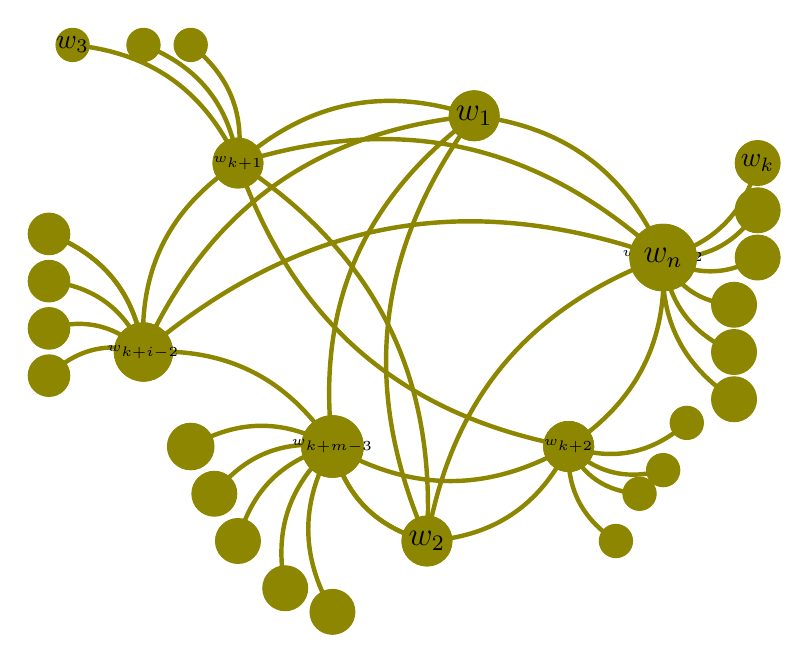
\begin{tikzpicture}[scale=0.3]

\draw[-,>=latex,ultra thick,color=olive] (14,2) to [bend left] (10,6);
\draw[-,>=latex,ultra thick,color=olive] (14,2) to [bend right] (20,6);
\draw[-,>=latex,ultra thick, color=olive] (10,6) to [bend right] (2,10);%
\draw[-,>=latex,ultra thick, color=olive] (2,10) to [bend left] (6,18);
\draw[-, >=latex,ultra thick, color=olive] (20,6) to [bend right] (24,14);%
\draw[-, >=latex,ultra thick, color=olive] (6,18) to [bend left] (16,20);
\draw[-, >=latex,ultra thick, color=olive] (16,20) to [bend left] (24,14); %

\draw[-, >=latex,ultra thick, color=olive] (16,20) to [bend right] (2,10);
\draw[-, >=latex,ultra thick, color=olive] (16,20) to [bend right] (10,6);
\draw[-, >=latex,ultra thick,color=olive] (6,18) to [bend left] (14,2);
\draw[-, >=latex,ultra thick, color=olive] (2,10) to [bend left] (24,14);%%
\draw[-,>=latex,ultra thick, color=olive] (10,6) to [bend right] (20,6);
\draw[-, >=latex,ultra thick,color=olive] (24,14) to [bend right] (14,2);
\draw[-,>=latex,ultra thick, color=olive] (16,20) to [bend right] (14,2);
\draw[-, >=latex,ultra thick,color=olive] (6,18) to [bend right] (20,6);
\draw[-, >=latex,ultra thick, color=olive] (6,18) to [bend left] (24,14);%
\draw[-, >=latex,ultra thick, color=olive] (10,6) to [bend right] (14,2);




\filldraw[color=olive] (14,2) circle (30pt) node[] {\large \textcolor{black}{$v_2$}};
\filldraw[color=olive] (10,6) circle (30pt)node[] {\large \textcolor{black}{\normalsize{$v_{6}$}}};;
 \filldraw[color=olive] (20,6) circle (30pt)node[] {\large \textcolor{black}{$v_4$}};;
 \filldraw[color=olive] (2,10) circle (25pt)node[] {\large \textcolor{black}{$v_5$}}; 
 \filldraw[color=olive] (6,18) circle (25pt)node[] {\large \textcolor{black}{$v_3$}};;
 \filldraw[color=olive] (24,14) circle (25pt)node[] {\large \textcolor{black}{$v_7$}};;
\filldraw[color=olive] (16,20) circle (30pt) node[] {\large \textcolor{black}{$v_1$}};


%%%%%%%%%%%%%%%%%%%%%%%%%%%%%%%%
\filldraw[color=olive] (16,20) circle (30pt) node[] {\large \textcolor{black}{$w_1$}};
%%%%%%%%%%%%%%%%%%%%%%%%%%%%%%%%%%%%%%%%%%%%%
\filldraw[color=olive] (14,2) circle (30pt) node[] {\large \textcolor{black}{$w_2$}};

%%%%%%%%%%%%%%%%%%%%%%%%%%%%%%%%%


\draw[-,>=latex,ultra thick,color=olive] (6,18) to [bend right](-1,23);
\draw[-,>=latex,ultra thick, color=olive] (6,18) to [bend right] (2,23);
\draw[-,>=latex,ultra thick, color=olive] (6,18) to [bend right] (4,23);

\filldraw[color=olive] (-1,23) circle (20pt) node[] {\textcolor{black}{$w_3$}};
\filldraw[color=olive] (2,23) circle (20pt);% node[] { \textcolor{black}{$w_4$}};
\filldraw[color=olive] (4,23) circle (20pt);% node[] {\textcolor{black}{$w_5$}};

\filldraw[color=olive] (6,18) circle (30pt) node[] { \textcolor{black}{$w_{25} $}};

%%%%%%%%%%%%%%%%%%%%%%%%%%%%%%%%%%%%%%

\draw[-,>=latex,ultra thick, color=olive] (20,6) to [bend right](22,2);
\draw[-, >=latex,ultra thick,color=olive] (20,6) to [bend right] (23,4);
\draw[-,>=latex,ultra thick, color=olive] (20,6) to [bend right] (24,5);
\draw[-,>=latex,ultra thick,color=olive] (20,6) to [bend right] (25,7);

\filldraw[color=olive] (22,2) circle (20pt);% node[] {\textcolor{black}{$w_6$}};
\filldraw[color=olive] (23,4) circle (20pt);% node[] { \textcolor{black}{$w_7$}};
\filldraw[color=olive] (24,5) circle (20pt);% node[] {\textcolor{black}{$w_8$}};
\filldraw[color=olive] (25,7) circle (20pt);% node[] { \textcolor{black}{$w_9$}};
%\filldraw[color=olive] (6,18) circle (20pt) node[] {\tiny \textcolor{black}{$w_{k+1}$}};
\filldraw[color=olive] (20,6) circle (30pt);% node[] {\textcolor{black}{$w_{26}$}};


%%%%%%%%%%%%%%%%%%%%%%%%%%%%%%%%%%%%%%55
\draw[-,>=latex,ultra thick,color=olive] (2,10) to [bend right](-2,9);
\draw[-,>=latex,ultra thick,color=olive] (2,10) to [bend right] (-2,11);
\draw[-,>=latex,ultra thick,color=olive] (2,10) to [bend right] (-2,13);
\draw[-,>=latex,ultra thick,color=olive] (2,10) to [bend right] (-2,15);
\draw[-,>=latex,ultra thick,color=olive] (2,10) to [bend right] (-2,15);

\filldraw[color=olive] (-2,9) circle (25pt);% node[] { \textcolor{black}{$w_{10}$}};
\filldraw[color=olive] (-2,11) circle (25pt);% node[] { \textcolor{black}{$w_{11}$}};
\filldraw[color=olive] (-2,13) circle (25pt);% node[] {\textcolor{black}{$w_{12}$}};
\filldraw[color=olive] (-2,15) circle (25pt);% node[] {\textcolor{black}{$w_{13}$}};


\filldraw[color=olive] (2,10) circle (35pt);% node[] {\textcolor{black}{$w_{27}$}};


%%%%%%%%%%%%%%%%%%%%%%%%%%%%%%%55

\draw[-,>=latex,ultra thick,color=olive] (10,6) to [bend right](10,-1);
\draw[-,>=latex,ultra thick,color=olive] (10,6) to [bend right] (8,0);
\draw[-,>=latex,ultra thick,color=olive] (10,6) to [bend right] (6,2);
\draw[-,>=latex,ultra thick,color=olive] (10,6) to [bend right] (5,4);
\draw[-,>=latex,ultra thick,color=olive] (10,6) to [bend right] (4,6);
\filldraw[color=olive] (10,-1) circle (27pt);% node[] { \textcolor{black}{$w_{14}$}};
\filldraw[color=olive] (8,0) circle (27pt); %node[] { \textcolor{black}{$w_{15}$}};
\filldraw[color=olive] (6,2) circle (27pt); %node[] { \textcolor{black}{$w_{16}$}};
\filldraw[color=olive] (5,4) circle (27pt); %node[]{ \textcolor{black}{$w_{17}$}};
\filldraw[color=olive] (4,6) circle (28pt);% node[] {\textcolor{black}{$w_{18}$}};





\filldraw[color=olive] (10,6) circle (37pt) node[] { \textcolor{black}{$w_{28}$}};

%%%%%%%%%%%%%%%%%%%%%%%%%%%%%%%%%%%%%%%%%%%%%%%%%%
\draw[-,>=latex,ultra thick, color=olive] (24,14) to [bend right](27,8);
\draw[-,>=latex,ultra thick,color=olive] (24,14) to [bend right] (27,10);
\draw[-,>=latex,ultra thick,color=olive] (24,14) to [bend right] (27,12);
\draw[-,>=latex,ultra thick,color=olive] (24,14) to [bend right] (28,14);
\draw[-,>=latex,ultra thick,color=olive] (24,14) to [bend right] (28,16);
\draw[-,>=latex,ultra thick,color=olive] (24,14) to [bend right] (28,18);

\filldraw[color=olive] (27,8) circle (27pt);% node[] { \textcolor{black}{$w_{19}$}};
\filldraw[color=olive] (27,10) circle (27pt);% node[] { \textcolor{black}{$w_{20}$}};
\filldraw[color=olive] (27,12) circle (27pt);%node[] { \textcolor{black}{$w_{21}$}};
\filldraw[color=olive] (28,14) circle (27pt);% node[] { \textcolor{black}{$w_{22}$}};
\filldraw[color=olive] (28,16) circle (27pt);% node[] { \textcolor{black}{$w_{23}$}};
\filldraw[color=olive] (28,18) circle (27pt) node[] {\textcolor{black}{$w_{k}$}};


\filldraw[color=olive] (6,18) circle (30pt) node[] {\tiny \textcolor{black}{$w_{k+1}$}};
\filldraw[color=olive] (20,6) circle (30pt) node[] {\tiny \textcolor{black}{$w_{k+2}$}};
\filldraw[color=olive] (2,10) circle (35pt) node[] {\tiny \textcolor{black}{$w_{k+i-2}$}};
\filldraw[color=olive] (10,6) circle (37pt) node[] {\tiny \textcolor{black}{$w_{k+m-3}$}};
\filldraw[color=olive] (24,14) circle (40pt) node[] {\tiny \textcolor{black}{$w_{k+m-2}$}};

\filldraw[color=olive] (24,14) circle (40pt) node[] {\large \textcolor{black}{$w_{n}$}};

\end{tikzpicture}
\end{center}
\end{figure}
\end{frame}